\documentclass{article}
\usepackage{tikz}
\usepackage{graphicx} % Required for inserting images
\usepackage{fullpage}
\usepackage{hyperref} % Required for inserting images
\usepackage{amsmath}
\usepackage{natbib}
\title{%Reduced asymptotic efficiency of
  Efficient
  cross-validation fold assignment with groups in multiple strata}
\author{Toby Hocking}
\date{April 2026}

\DeclareMathOperator*{\argmin}{arg\, min} 
\DeclareMathOperator*{\argmax}{arg\, max} 
\begin{document}

\maketitle

\begin{abstract}
    Cross-validation is used throughout machine learning for model training and evaluation. In classification data sets, stratification is used to ensure that splits preserve class proportions. In structured data (image segmentation, medical visits, etc.), grouping is used to prevent data leakage (data from the same group should not appear in both train and test sets). Fold assignment is trivial with either stratification or grouping, but it is NP-hard with both stratification and grouping. Scikit-learn implements a heuristic that obtains reasonable fold assignments in this case, but its time and memory complexity can be prohibitive for large data. We propose a new heuristic algorithm with asymptotically less time and memory usage, that can be used on large data sets. In an empirical analysis of 4 real data sets, the proposed algorithm provides comparable fold assignments, and is at least ten times faster than the previous algorithm.
\end{abstract} 



% Let there be $S$ strata in $K$-fold CV.
% Let $c = [c_1, \dots, c_S ]$ be strata counts for the next group --- it should be assigned to which fold $k$?
% \begin{eqnarray}
% \text{OldRSS}=
% &\sum_{\sigma\in\{1,\dots,S\}}&
% \sum_{\phi\in\{1,\dots,K\}}
% (\overbrace{\hat n_{\sigma,\phi}}^{\text{actual}} - \overbrace{n^*_\sigma}^{\text{ideal}})^2
% \\
% \text{NewRSS} = \min_{k\in\{1,\dots,K\}}
% &\sum_{\sigma\in\{1,\dots,S\}}&
% \sum_{\phi\in\{1,\dots,K\}}
% \big(
% (\hat n_{\sigma,\phi}+c_\sigma I[\phi=k]) - n^*_\sigma\big)^2
% \\
% \text{NewRSS} = \text{OldRSS} + \min_{k\in\{1,\dots,K\}}
% &\sum_{\sigma\in\{1,\dots,S\}}&
% c_\sigma ( 2 \hat n_{\sigma,k} +
% \underbrace{c_\sigma - 2n^*_\sigma}_{\text{no $k$}} 
% )
% \\
% k^* = 
% \argmin_{k\in\{1,\dots,K\}}
% &\sum_{\sigma\in\{1,\dots,S\}}&
% c_\sigma \hat n_{\sigma,k}
% \end{eqnarray}


Similar to 
\url{https://en.wikipedia.org/wiki/Bin_packinc_problem}
but with a fixed number of bins.

Quoting from that article:
``In the bin packing problem, the size of the bins is fixed and their number can be enlarged (but should be as small as possible).
In the multiway number partitioning problem, \url{https://en.wikipedia.org/wiki/Multiway_number_partitioning} the number of bins is fixed and their size can be enlarged.''
\citet{Pop2013} proposed a heuristic (genetic algorithm and local search) to solve this multidimensional multi-way number partitioning problem.

\citet{hayes2002computing} called it the ``easiest hard problem'' and discussed the example of picking team members in a game like soccer. 

\section{Introduction}
Medical data (respiratory in R), each patient is a group.

Satellite image segmentation, each labeled region is a group.

Pet adoption data, each rescuer is a group.

\subsection{Contributions}

Complexity analysis of previous Wasikowski algorthm in terms of two sub-routines, Sort() and get best fold().

Proposed online counting and group assignment algorithm, for asymptotically less memory usage.
Drops a potentially large $O(SG)$ term from memory complexity.

Proposed RSS minimization algorithm which is asymptotically faster: previous quadratic time in number of folds $K$ is reduced to linear time.

Systematic comparisons with 8 previous software packages, in terms of features and fold assignment accuracy.

\section{Related Work}

Wasikowski (sklearn.model\_selection.StratifiedGroupKFold) 

\begin{table}[t]
  \centering
  %\small
  \begin{tabular}{ccccccc}
             &       &        &        &           &           & group\\
             &       &        &        & 1 stratum & 2+ strata & +stratum\\
    Software & group & strata & subset & per group & per group &  +subset\\
    \hline
mlr3&yes&yes&no&no&no&no\\
caret&yes&yes&no&no&no&no\\
splitTools&yes&yes&no&no&no&no\\
origami&yes&yes&no&random+leakage&no&no\\
rsample&yes&yes&no&random&no&no\\
bioLeak&yes&yes&no&random&random&no\\
sklearn&yes&yes&no&yes&yes&no\\
soakpy&no&no&yes&no&no&no\\
\textbf{mlr3resampling}&yes&yes&yes&yes&yes&yes
  \end{tabular}
  \caption{Comparing features provided by previous software, and proposed \textbf{mlr3resampling} R package.}
  \label{tab:related}
\end{table}
\section{Proposed Methods}

Assume we have a data set with $N$ rows in $S$ strata and $G$ groups.
We want to perform $K$-fold cross-validation, such that data in each group are assigned the same fold ID, and the strata proportions in each fold are approximately equal.

For each row $i\in\{1,\dots,N\}$, we have a stratum $s_i\in\{1,\dots,S\}$, and a group $g_i\in\{1,\dots,G\}$.
The algorithm begins by counting the number of data in each stratum, then dividing by the number of folds, to obtain the ideal number of data.
For each stratum $\sigma\in\{1,\dots,S\}$, the ideal number of data is
\begin{equation}
n^*_\sigma = \sum_{i\in\{1,\dots,N\}}
I[s_i = \sigma]/K,
\end{equation}
where $I[\cdot]$ is the indicator function (1 if argument is true, 0 otherwise).

For each stratum $\sigma$ and fold $\phi\in\{1,\dots,K\}$, let $\hat n_{\sigma,\phi}$ be the number of data with that stratum assigned to that fold.
The optimization problem is to find a fold assignment which minimizes the residual sum of squares,
\begin{equation}
\text{RSS}=
\sum_{\sigma\in\{1,\dots,S\}}
\sum_{\phi\in\{1,\dots,K\}}
(\hat n_{\sigma,\phi} - n^*_\sigma)^2.
\end{equation}

We propose a greedy algorithm that computes an approximate solution in linear time (Table~\ref{tab:complexity}).
The algorithm starts with all $\hat n_{\sigma,\phi}=0$ and then assigns a fold to one group at a time.
Let $c_1,\dots,c_S $ be the counts of data in each stratum for the current group.
The problem is to decide the fold assignment for this group,
\begin{equation}
\min_{k\in\{1,\dots,K\}}
\sum_{\sigma\in\{1,\dots,S\}}
\sum_{\phi\in\{1,\dots,K\}}
\big(
(\hat n_{\sigma,\phi}+c_\sigma I[\phi=k]) - n^*_\sigma\big)^2.
\end{equation}
Expanding the square and simplifying yields
\begin{equation}
\min_{k\in\{1,\dots,K\}}
\sum_{\sigma\in\{1,\dots,S\}}
\sum_{\phi\in\{1,\dots,K\}}
\hat n^2_{\sigma,\phi}
- 2 \hat n_{\sigma,\phi} n^*_\sigma
+ {n^*_\sigma}^2
+ I[\phi=k] c_\sigma ( 2 \hat n_{\sigma,\phi} + c_\sigma - 2n^*_\sigma ).
\end{equation}
The first three terms above are the current RSS, which does not depend on $k$, so it is a constant that we can remove from the optimization problem.
Furthermore, the indicator function cancels the sum over folds $\phi$, yielding
\begin{equation}
\text{RSS} + \min_{k\in\{1,\dots,K\}}
\sum_{\sigma\in\{1,\dots,S\}}
c_\sigma ( 2 \hat n_{\sigma,k} + c_\sigma - 2n^*_\sigma ),
\end{equation}
% Simplifying yields
% \begin{equation}
% \text{RSS} + \min_{k\in\{1,\dots,K\}}
% \sum_{\sigma\in\{1,\dots,S\}}
% c_\sigma\big(c_\sigma+2(\hat n_{\sigma,k}-n^*_\sigma)\big),
% \end{equation}
which is a simple update rule that can be used to obtain an efficient algorithm.
Taking the argmin, we can remove the terms that do not depend on $k$, yielding
\begin{equation}
  \label{eq:k*}
k^* = 
\argmin_{k\in\{1,\dots,K\}}
\sum_{\sigma\in\{1,\dots,S\}}
c_\sigma \hat n_{\sigma,k}.
\end{equation}
\subsection{Complexity analysis}
We assume there are $N$ data, $K$ folds, $G$ groups, and $S$ strata.
All algorithms begin by sorting the groups, typically $O(N\log N)$ time.

The previous Wasikowski algorithm begins by computing a $G\times S$ matrix of counts per group and stratum, requiring $O(GS)$ time and memory.
For large $G$ and $S$, this large count matrix will be very sparse (almost all entries zero), which is inefficient.
Because the large size of this matrix could be prohibitive, we propose to modify the Wasikowski algorithm to avoid this inefficiency.
Our proposed memory-efficient variant is called Wasikowski-L in Table~\ref{tab:complexity} (L for Limited memory).
We propose to first sort the data by group, then compute and store a count vector for only the current group, thus reducing the memory requirement to $O(S)$, which can be ignored since it is smaller than $O(N)$ (Table~\ref{tab:complexity}, proposed rows, Memory column).

The previous Wasikowski algorithm maintains a $K\times S$ matrix of counts per fold and stratum.
The \texttt{get\_best\_fold()} method considers putting the new group in each of the $K$ folds, then computes SD over folds for each stratum, then mean of SD values over strata.
The \texttt{get\_best\_fold()} method is therefore $O(K^2 S)$ time, and the overall algorithm is therefore $O(N\log N + K^2 G S)$ time (Table~\ref{tab:complexity}, Wasikowski rows, Time column).

The proposed RSS minimization procedure~(\ref{eq:k*}) has a sum over $S$ terms inside a min over $K$ terms.
The proposed \texttt{get\_best\_fold()} is therefore $O(SK)$ time.
Comparing to the previous Wasikowski algorthm, the proposed RSS minimization is asymptotically faster (linear rather than quadratic in the number of folds $K$).
The overall time complexity of the proposed RSS minimization algorithm is therefore

TODO pseudo-code.

\begin{verbatim}
def assign_folds(strata, groups, N_folds):
  count_matrix = zeros(N_strata, N_folds)
  folds = []
  for group in Sort(groups):
    best_fold = get_best_fold(group)
    count_matrix[, best_fold] += get_count(group)
    folds.append(group, best_fold)
  return folds
\end{verbatim}

\subsection{Simple example where RSS beats Wasikowski}

\begin{verbatim}
   counts  fold   rss
1:    1,3     1     0
2:    1,2     2     1
3:    0,2     3     2
4:    1,1     3     4
5:    0,1     2     5
   fold
y   1 2 3
  1 1 1 1
  2 3 3 3
   counts  fold   var g_ord
1:    0,2     1   2.0     1
2:    1,3     2   2.0     6
3:    1,2     3   0.5     2
4:    0,1     1   0.5     8
5:    1,1     1   0.0     4
   fold
y   1 2 3
  1 1 1 1
  2 4 3 2
\end{verbatim}

\subsection{Tie-breaking}
\begin{verbatim}
Example: 6 groups, 2-fold CV.
     group   rss  nrow  freq
 1:    5,3     5     8  22.5
 2:    3,0    34     3   9.0
 3:    1,2    34     3   8.0
 4:    1,2    34     3   8.0
 5:    1,2    34     3   8.0
 6:    1,1    41     2   5.5
TOTAL 12,10
ideal  6,5    
\end{verbatim}

\begin{verbatim}
freq = mean(ideal*group)
-Prefer groups with more
 data in larger strata.
\end{verbatim}

\begin{verbatim}
     group  fold  fold1  fold2
1:    5,3     1    5,3    0,0
2:    1,2     2    5,3    1,2
3:    1,2     2    5,3    2,4
4:    1,2     2    5,3    3,6
5:    3,0     2    5,3    6,6
6:    1,1     1    6,4    6,6
3,0 added near end = Not ideal!    
\end{verbatim}

\begin{verbatim}
1:    5,3     1    5,3    0,0
2:    3,0     2    5,3    3,0
3:    1,2     2    5,3    4,2
4:    1,2     2    5,3    5,4
5:    1,2     1    6,5    5,4
6:    1,1     2    6,5    6,5
3,0 added first =  Yes ideal!
\end{verbatim}



\verb|bioLeak::make_split_plan|
stratify: logical, keep outcome proportions similar across folds. For
          grouped modes, stratification is applied at the group level
          (by majority class per group) if 'outcome' is provided;
          otherwise ignored.

\begin{table}[t]
    \centering
    \begin{tabular}{c|c|l}
        Algorithm &  Time    & Memory \\
        \hline
        Wasikowski & $O(N\log N + K^2GS)$ & $O(N + SK+SG)$\\
        Wasikowski-L (proposed) & $O(N\log N + K^2GS)$ & $O(N + SK)$\\
        %MinRSS (proposed) & $O(N + KGS)$  & $O(N + SK + SG)$\\
        MinRSS (proposed) & $O(N\log N + KGS)$  & $O(N + SK)$
    \end{tabular}
    \caption{Time and memory complexity for computing $K$-fold cross-validation assignment, given $N$ data rows in $S$ strata and $G$ groups.}
    \label{tab:complexity}
\end{table}

\begin{figure}[t]
    \centering
    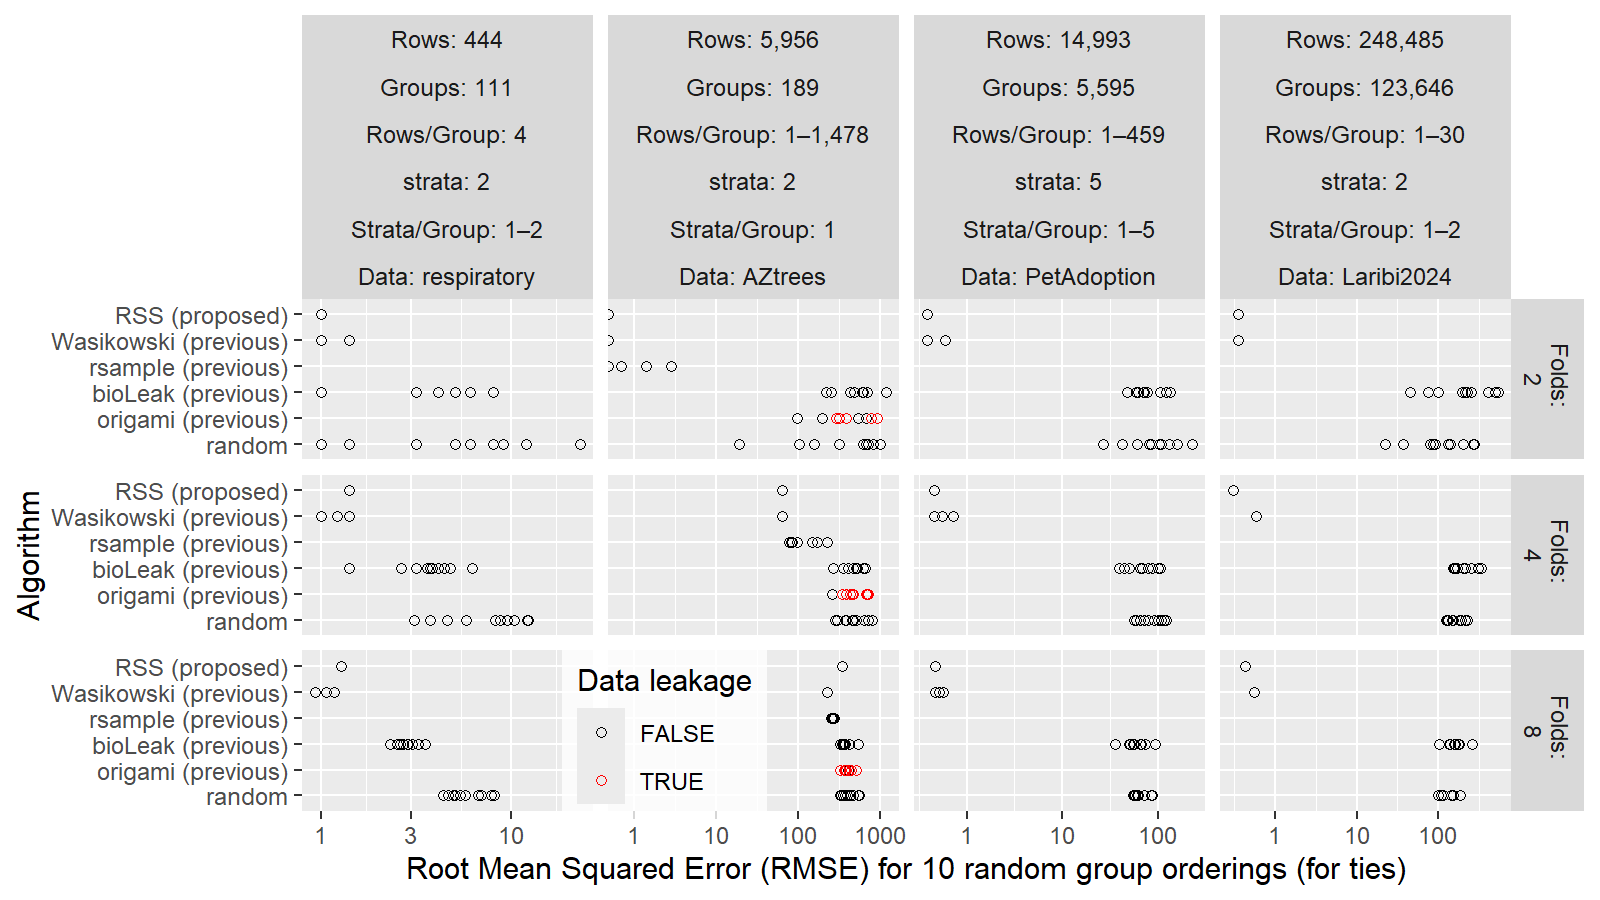
\includegraphics[width=\linewidth]{several_Tasks_even.png}
    \caption{Caption}
    \label{fig:several_Tasks}
\end{figure}

\begin{figure}[t]
    \centering
    % 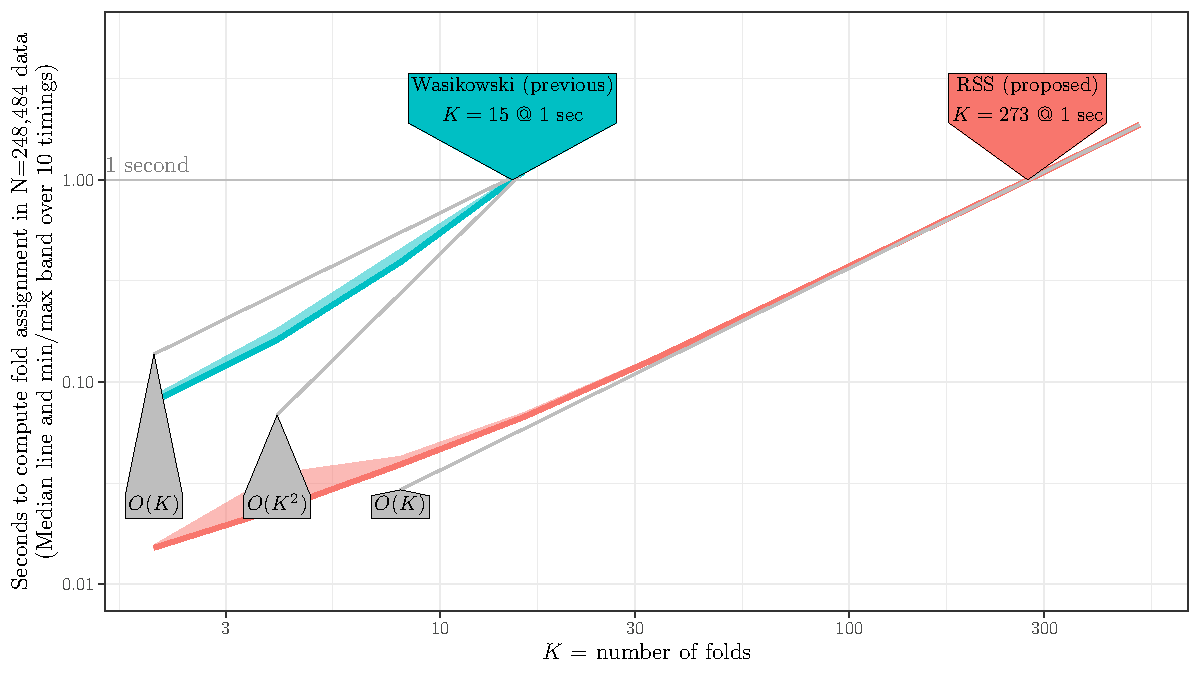
\includegraphics[width=\linewidth]{Laribi2024-figure-refs}
    % Created by tikzDevice version 0.12.6 on 2026-06-17 14:28:33
% !TEX encoding = UTF-8 Unicode
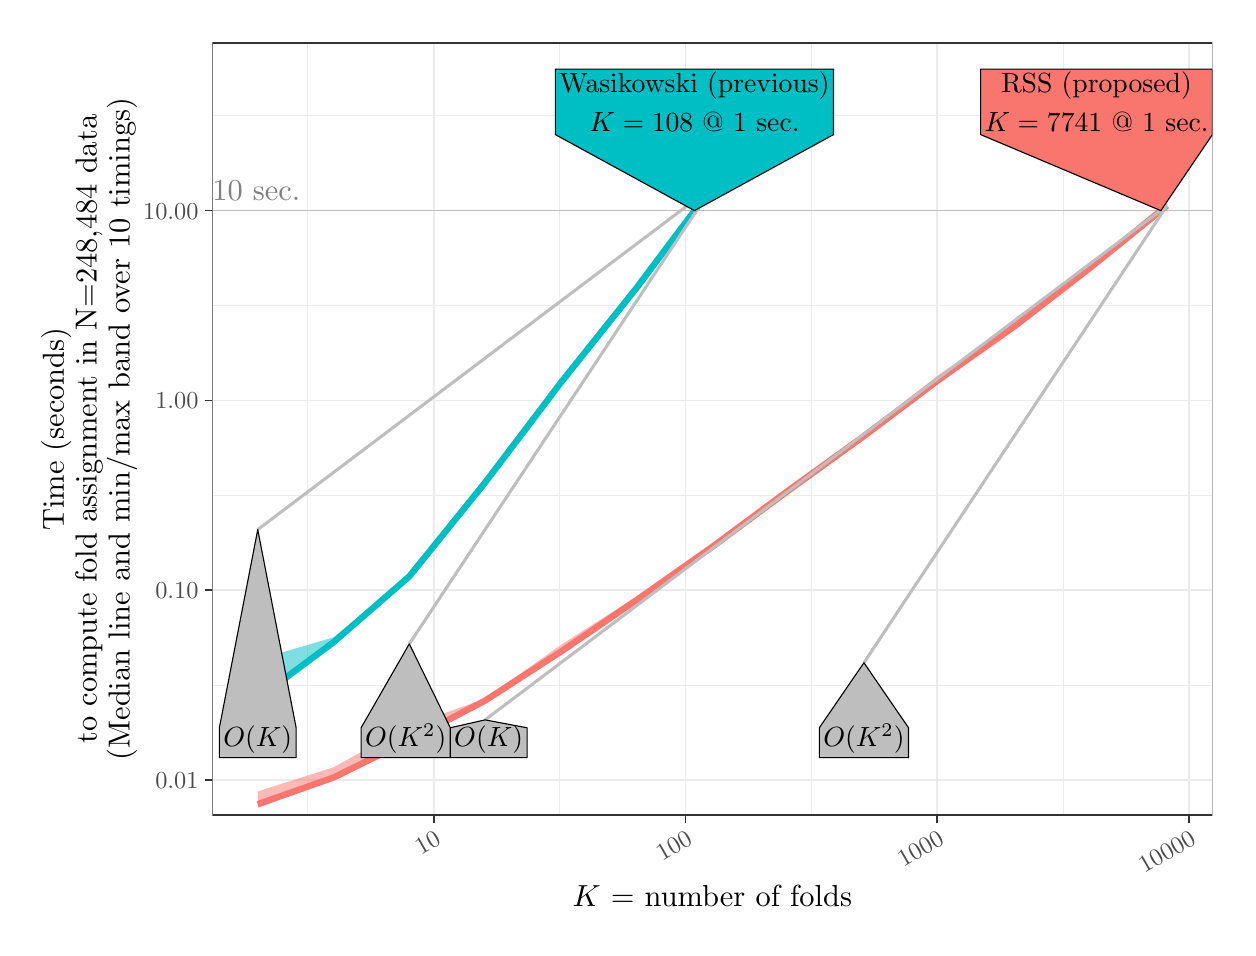
\begin{tikzpicture}[x=1pt,y=1pt]
\definecolor{fillColor}{RGB}{255,255,255}
\path[use as bounding box,fill=fillColor,fill opacity=0.00] (0,0) rectangle (433.62,325.21);
\begin{scope}
\path[clip] (  0.00,  0.00) rectangle (433.62,325.21);
\definecolor{drawColor}{RGB}{255,255,255}
\definecolor{fillColor}{RGB}{255,255,255}

\path[draw=drawColor,line width= 0.6pt,line join=round,line cap=round,fill=fillColor] (  0.00,  0.00) rectangle (433.62,325.21);
\end{scope}
\begin{scope}
\path[clip] ( 66.71, 40.64) rectangle (428.12,319.71);
\definecolor{fillColor}{RGB}{255,255,255}

\path[fill=fillColor] ( 66.71, 40.64) rectangle (428.12,319.71);
\definecolor{drawColor}{gray}{0.92}

\path[draw=drawColor,line width= 0.3pt,line join=round] ( 66.71, 87.62) --
	(428.12, 87.62);

\path[draw=drawColor,line width= 0.3pt,line join=round] ( 66.71,156.21) --
	(428.12,156.21);

\path[draw=drawColor,line width= 0.3pt,line join=round] ( 66.71,224.80) --
	(428.12,224.80);

\path[draw=drawColor,line width= 0.3pt,line join=round] ( 66.71,293.38) --
	(428.12,293.38);

\path[draw=drawColor,line width= 0.3pt,line join=round] (101.24, 40.64) --
	(101.24,319.71);

\path[draw=drawColor,line width= 0.3pt,line join=round] (192.19, 40.64) --
	(192.19,319.71);

\path[draw=drawColor,line width= 0.3pt,line join=round] (283.14, 40.64) --
	(283.14,319.71);

\path[draw=drawColor,line width= 0.3pt,line join=round] (374.09, 40.64) --
	(374.09,319.71);

\path[draw=drawColor,line width= 0.6pt,line join=round] ( 66.71, 53.33) --
	(428.12, 53.33);

\path[draw=drawColor,line width= 0.6pt,line join=round] ( 66.71,121.91) --
	(428.12,121.91);

\path[draw=drawColor,line width= 0.6pt,line join=round] ( 66.71,190.50) --
	(428.12,190.50);

\path[draw=drawColor,line width= 0.6pt,line join=round] ( 66.71,259.09) --
	(428.12,259.09);

\path[draw=drawColor,line width= 0.6pt,line join=round] (146.71, 40.64) --
	(146.71,319.71);

\path[draw=drawColor,line width= 0.6pt,line join=round] (237.67, 40.64) --
	(237.67,319.71);

\path[draw=drawColor,line width= 0.6pt,line join=round] (328.62, 40.64) --
	(328.62,319.71);

\path[draw=drawColor,line width= 0.6pt,line join=round] (419.57, 40.64) --
	(419.57,319.71);
\definecolor{drawColor}{gray}{0.50}

\node[text=drawColor,anchor=base west,inner sep=0pt, outer sep=0pt, scale=  1.10] at ( 66.71,262.88) { 10 sec.};
\definecolor{drawColor}{RGB}{190,190,190}

\path[draw=drawColor,line width= 0.6pt,line join=round] ( 66.71,259.09) -- (428.12,259.09);
\definecolor{fillColor}{RGB}{248,118,109}

\path[fill=fillColor,fill opacity=0.50] ( 83.14, 49.23) --
	(110.52, 57.94) --
	(137.90, 73.01) --
	(165.28, 82.72) --
	(192.66,102.15) --
	(220.04,119.69) --
	(247.42,138.58) --
	(274.80,158.71) --
	(302.18,178.64) --
	(329.55,200.00) --
	(356.93,218.66) --
	(384.31,239.01) --
	(411.69,261.83) --
	(411.69,260.23) --
	(384.31,237.76) --
	(356.93,216.81) --
	(329.55,197.65) --
	(302.18,177.17) --
	(274.80,156.60) --
	(247.42,137.06) --
	(220.04,117.58) --
	(192.66, 99.05) --
	(165.28, 81.55) --
	(137.90, 67.33) --
	(110.52, 53.80) --
	( 83.14, 43.29) --
	cycle;

\path[] ( 83.14, 49.23) --
	(110.52, 57.94) --
	(137.90, 73.01) --
	(165.28, 82.72) --
	(192.66,102.15) --
	(220.04,119.69) --
	(247.42,138.58) --
	(274.80,158.71) --
	(302.18,178.64) --
	(329.55,200.00) --
	(356.93,218.66) --
	(384.31,239.01) --
	(411.69,261.83);

\path[] (411.69,260.23) --
	(384.31,237.76) --
	(356.93,216.81) --
	(329.55,197.65) --
	(302.18,177.17) --
	(274.80,156.60) --
	(247.42,137.06) --
	(220.04,117.58) --
	(192.66, 99.05) --
	(165.28, 81.55) --
	(137.90, 67.33) --
	(110.52, 53.80) --
	( 83.14, 43.29);
\definecolor{fillColor}{RGB}{0,191,196}

\path[fill=fillColor,fill opacity=0.50] ( 83.14, 96.87) --
	(110.52,104.91) --
	(137.90,127.24) --
	(165.28,161.72) --
	(192.66,197.57) --
	(220.04,231.73) --
	(247.42,268.22) --
	(247.42,267.07) --
	(220.04,230.59) --
	(192.66,196.24) --
	(165.28,160.23) --
	(137.90,126.33) --
	(110.52,102.44) --
	( 83.14, 82.18) --
	cycle;

\path[] ( 83.14, 96.87) --
	(110.52,104.91) --
	(137.90,127.24) --
	(165.28,161.72) --
	(192.66,197.57) --
	(220.04,231.73) --
	(247.42,268.22);

\path[] (247.42,267.07) --
	(220.04,230.59) --
	(192.66,196.24) --
	(165.28,160.23) --
	(137.90,126.33) --
	(110.52,102.44) --
	( 83.14, 82.18);
\definecolor{drawColor}{RGB}{248,118,109}

\path[draw=drawColor,line width= 2.3pt,line join=round] ( 83.14, 44.61) --
	(110.52, 54.25) --
	(137.90, 67.71) --
	(165.28, 82.04) --
	(192.66, 99.73) --
	(220.04,118.37) --
	(247.42,137.63) --
	(274.80,157.90) --
	(302.18,177.62) --
	(329.55,198.20) --
	(356.93,217.54) --
	(384.31,238.73) --
	(411.69,260.90);
\definecolor{drawColor}{RGB}{0,191,196}

\path[draw=drawColor,line width= 2.3pt,line join=round] ( 83.14, 82.75) --
	(110.52,103.14) --
	(137.90,126.92) --
	(165.28,160.83) --
	(192.66,196.94) --
	(220.04,231.21) --
	(247.42,267.72);
\definecolor{drawColor}{RGB}{190,190,190}

\path[draw=drawColor,line width= 1.1pt,line join=round] (165.28, 75.08) --
	(192.66, 95.72) --
	(220.04,116.37) --
	(247.42,137.02) --
	(274.80,157.67) --
	(302.18,178.31) --
	(329.55,198.96) --
	(356.93,219.61) --
	(384.31,240.25) --
	(411.69,260.90);

\path[draw=drawColor,line width= 1.1pt,line join=round] (302.18, 95.72) --
	(329.55,137.02) --
	(356.93,178.31) --
	(384.31,219.61) --
	(411.69,260.90);

\path[draw=drawColor,line width= 1.1pt,line join=round] ( 83.14,143.84) --
	(110.52,164.49) --
	(137.90,185.14) --
	(165.28,205.78) --
	(192.66,226.43) --
	(220.04,247.08) --
	(247.42,267.72);

\path[draw=drawColor,line width= 1.1pt,line join=round] (137.90,102.55) --
	(165.28,143.84) --
	(192.66,185.14) --
	(220.04,226.43) --
	(247.42,267.72);
\end{scope}
\begin{scope}
\path[clip] ( 66.71, 40.64) rectangle (428.12,319.71);
\definecolor{drawColor}{RGB}{0,0,0}
\definecolor{fillColor}{RGB}{248,118,109}

\path[draw=drawColor,line width= 0.4pt,line join=round,line cap=round,fill=fillColor] (344.35,310.25) --
	(428.12,310.25) --
	(428.12,286.57) --
	(409.46,259.09) --
	(344.35,286.57) --
	cycle;
\definecolor{fillColor}{RGB}{0,191,196}

\path[draw=drawColor,line width= 0.4pt,line join=round,line cap=round,fill=fillColor] (190.68,310.25) --
	(291.20,310.25) --
	(291.20,286.57) --
	(240.94,259.09) --
	(190.68,286.57) --
	cycle;

\node[text=drawColor,anchor=base,inner sep=0pt, outer sep=0pt, scale=  1.00] at (386.24,301.94) {RSS (proposed)};

\node[text=drawColor,anchor=base,inner sep=0pt, outer sep=0pt, scale=  1.00] at (386.24,287.54) {$K=7741$ @ 1 sec.};

\node[text=drawColor,anchor=base,inner sep=0pt, outer sep=0pt, scale=  1.00] at (240.94,301.94) {Wasikowski (previous)};

\node[text=drawColor,anchor=base,inner sep=0pt, outer sep=0pt, scale=  1.00] at (240.94,287.54) {$K=108$ @ 1 sec.};
\end{scope}
\begin{scope}
\path[clip] ( 66.71, 40.64) rectangle (428.12,319.71);
\definecolor{drawColor}{RGB}{0,0,0}
\definecolor{fillColor}{RGB}{190,190,190}

\path[draw=drawColor,line width= 0.4pt,line join=round,line cap=round,fill=fillColor] (152.71, 72.23) --
	(165.28, 75.08) --
	(180.45, 72.23) --
	(180.45, 61.42) --
	(152.71, 61.42) --
	cycle;

\path[draw=drawColor,line width= 0.4pt,line join=round,line cap=round,fill=fillColor] ( 69.27, 72.23) --
	( 83.14,143.84) --
	( 97.01, 72.23) --
	( 97.01, 61.42) --
	( 69.27, 61.42) --
	cycle;

\path[draw=drawColor,line width= 0.4pt,line join=round,line cap=round,fill=fillColor] (286.06, 72.23) --
	(302.18, 95.72) --
	(318.29, 72.23) --
	(318.29, 61.42) --
	(286.06, 61.42) --
	cycle;

\path[draw=drawColor,line width= 0.4pt,line join=round,line cap=round,fill=fillColor] (120.49, 72.23) --
	(137.90,102.55) --
	(152.71, 72.23) --
	(152.71, 61.42) --
	(120.49, 61.42) --
	cycle;

\node[text=drawColor,anchor=base,inner sep=0pt, outer sep=0pt, scale=  1.00] at (166.58, 65.35) {$O(K)$};

\node[text=drawColor,anchor=base,inner sep=0pt, outer sep=0pt, scale=  1.00] at ( 83.14, 65.35) {$O(K)$};

\node[text=drawColor,anchor=base,inner sep=0pt, outer sep=0pt, scale=  1.00] at (302.18, 65.35) {$O(K^2)$};

\node[text=drawColor,anchor=base,inner sep=0pt, outer sep=0pt, scale=  1.00] at (136.60, 65.35) {$O(K^2)$};
\definecolor{drawColor}{gray}{0.20}

\path[draw=drawColor,line width= 0.6pt,line join=round,line cap=round] ( 66.71, 40.64) rectangle (428.12,319.71);
\end{scope}
\begin{scope}
\path[clip] (  0.00,  0.00) rectangle (433.62,325.21);
\definecolor{drawColor}{gray}{0.30}

\node[text=drawColor,anchor=base east,inner sep=0pt, outer sep=0pt, scale=  0.88] at ( 61.76, 50.30) {0.01};

\node[text=drawColor,anchor=base east,inner sep=0pt, outer sep=0pt, scale=  0.88] at ( 61.76,118.88) {0.10};

\node[text=drawColor,anchor=base east,inner sep=0pt, outer sep=0pt, scale=  0.88] at ( 61.76,187.47) {1.00};

\node[text=drawColor,anchor=base east,inner sep=0pt, outer sep=0pt, scale=  0.88] at ( 61.76,256.06) {10.00};
\end{scope}
\begin{scope}
\path[clip] (  0.00,  0.00) rectangle (433.62,325.21);
\definecolor{drawColor}{gray}{0.20}

\path[draw=drawColor,line width= 0.6pt,line join=round] ( 63.96, 53.33) --
	( 66.71, 53.33);

\path[draw=drawColor,line width= 0.6pt,line join=round] ( 63.96,121.91) --
	( 66.71,121.91);

\path[draw=drawColor,line width= 0.6pt,line join=round] ( 63.96,190.50) --
	( 66.71,190.50);

\path[draw=drawColor,line width= 0.6pt,line join=round] ( 63.96,259.09) --
	( 66.71,259.09);
\end{scope}
\begin{scope}
\path[clip] (  0.00,  0.00) rectangle (433.62,325.21);
\definecolor{drawColor}{gray}{0.20}

\path[draw=drawColor,line width= 0.6pt,line join=round] (146.71, 37.89) --
	(146.71, 40.64);

\path[draw=drawColor,line width= 0.6pt,line join=round] (237.67, 37.89) --
	(237.67, 40.64);

\path[draw=drawColor,line width= 0.6pt,line join=round] (328.62, 37.89) --
	(328.62, 40.64);

\path[draw=drawColor,line width= 0.6pt,line join=round] (419.57, 37.89) --
	(419.57, 40.64);
\end{scope}
\begin{scope}
\path[clip] (  0.00,  0.00) rectangle (433.62,325.21);
\definecolor{drawColor}{gray}{0.30}

\node[text=drawColor,rotate= 30.00,anchor=base east,inner sep=0pt, outer sep=0pt, scale=  0.88] at (149.74, 30.44) {10};

\node[text=drawColor,rotate= 30.00,anchor=base east,inner sep=0pt, outer sep=0pt, scale=  0.88] at (240.70, 30.44) {100};

\node[text=drawColor,rotate= 30.00,anchor=base east,inner sep=0pt, outer sep=0pt, scale=  0.88] at (331.65, 30.44) {1000};

\node[text=drawColor,rotate= 30.00,anchor=base east,inner sep=0pt, outer sep=0pt, scale=  0.88] at (422.60, 30.44) {10000};
\end{scope}
\begin{scope}
\path[clip] (  0.00,  0.00) rectangle (433.62,325.21);
\definecolor{drawColor}{RGB}{0,0,0}

\node[text=drawColor,anchor=base,inner sep=0pt, outer sep=0pt, scale=  1.10] at (247.42,  7.64) {$K$ = number of folds};
\end{scope}
\begin{scope}
\path[clip] (  0.00,  0.00) rectangle (433.62,325.21);
\definecolor{drawColor}{RGB}{0,0,0}

\node[text=drawColor,rotate= 90.00,anchor=base,inner sep=0pt, outer sep=0pt, scale=  1.10] at ( 13.08,180.18) {Time (seconds)};

\node[text=drawColor,rotate= 90.00,anchor=base,inner sep=0pt, outer sep=0pt, scale=  1.10] at ( 24.96,180.18) {to compute fold assignment in N=248,484 data};

\node[text=drawColor,rotate= 90.00,anchor=base,inner sep=0pt, outer sep=0pt, scale=  1.10] at ( 36.84,180.18) {(Median line and min/max band over 10 timings)};
\end{scope}
\end{tikzpicture}

    \caption{Caption}
    \label{fig:Laribi-refs}
\end{figure}

\begin{figure}[t]
    \centering
    % 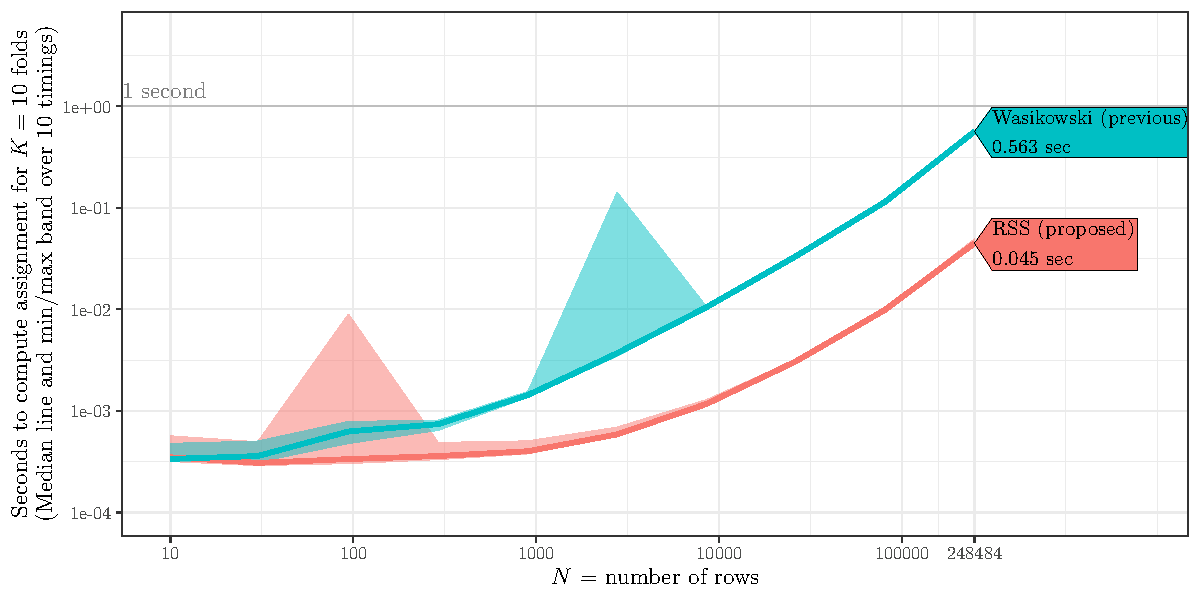
\includegraphics[width=\linewidth]{Laribi2024-figure-rows}
    % Created by tikzDevice version 0.12.6 on 2026-06-17 14:28:46
% !TEX encoding = UTF-8 Unicode
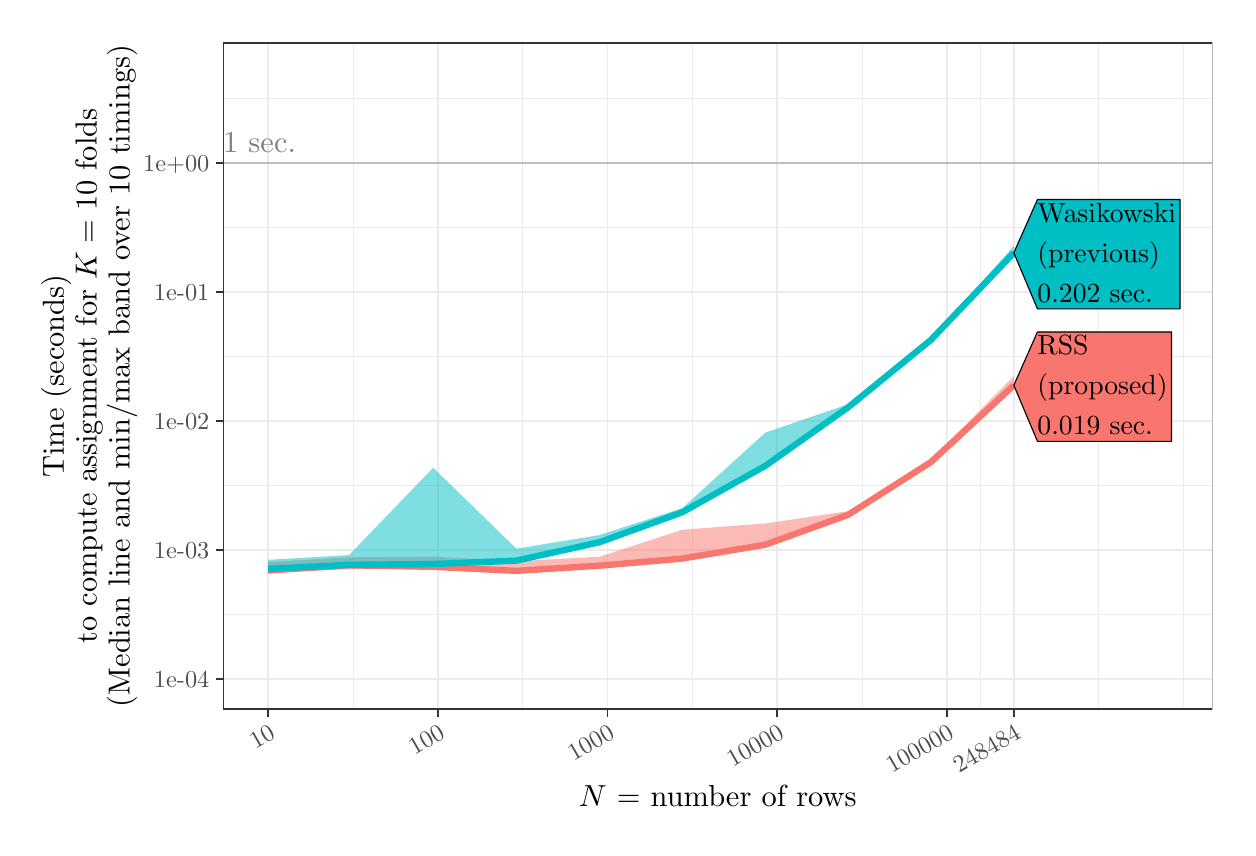
\begin{tikzpicture}[x=1pt,y=1pt]
\definecolor{fillColor}{RGB}{255,255,255}
\path[use as bounding box,fill=fillColor,fill opacity=0.00] (0,0) rectangle (433.62,289.08);
\begin{scope}
\path[clip] (  0.00,  0.00) rectangle (433.62,289.08);
\definecolor{drawColor}{RGB}{255,255,255}
\definecolor{fillColor}{RGB}{255,255,255}

\path[draw=drawColor,line width= 0.6pt,line join=round,line cap=round,fill=fillColor] (  0.00,  0.00) rectangle (433.62,289.08);
\end{scope}
\begin{scope}
\path[clip] ( 70.62, 42.84) rectangle (428.12,283.58);
\definecolor{fillColor}{RGB}{255,255,255}

\path[fill=fillColor] ( 70.62, 42.84) rectangle (428.12,283.58);
\definecolor{drawColor}{gray}{0.92}

\path[draw=drawColor,line width= 0.3pt,line join=round] ( 70.62, 77.07) --
	(428.12, 77.07);

\path[draw=drawColor,line width= 0.3pt,line join=round] ( 70.62,123.65) --
	(428.12,123.65);

\path[draw=drawColor,line width= 0.3pt,line join=round] ( 70.62,170.22) --
	(428.12,170.22);

\path[draw=drawColor,line width= 0.3pt,line join=round] ( 70.62,216.80) --
	(428.12,216.80);

\path[draw=drawColor,line width= 0.3pt,line join=round] ( 70.62,263.37) --
	(428.12,263.37);

\path[draw=drawColor,line width= 0.3pt,line join=round] (117.53, 42.84) --
	(117.53,283.58);

\path[draw=drawColor,line width= 0.3pt,line join=round] (178.84, 42.84) --
	(178.84,283.58);

\path[draw=drawColor,line width= 0.3pt,line join=round] (240.14, 42.84) --
	(240.14,283.58);

\path[draw=drawColor,line width= 0.3pt,line join=round] (301.45, 42.84) --
	(301.45,283.58);

\path[draw=drawColor,line width= 0.3pt,line join=round] (344.22, 42.84) --
	(344.22,283.58);

\path[draw=drawColor,line width= 0.3pt,line join=round] (387.00, 42.84) --
	(387.00,283.58);

\path[draw=drawColor,line width= 0.3pt,line join=round] (417.65, 42.84) --
	(417.65,283.58);

\path[draw=drawColor,line width= 0.6pt,line join=round] ( 70.62, 53.78) --
	(428.12, 53.78);

\path[draw=drawColor,line width= 0.6pt,line join=round] ( 70.62,100.36) --
	(428.12,100.36);

\path[draw=drawColor,line width= 0.6pt,line join=round] ( 70.62,146.93) --
	(428.12,146.93);

\path[draw=drawColor,line width= 0.6pt,line join=round] ( 70.62,193.51) --
	(428.12,193.51);

\path[draw=drawColor,line width= 0.6pt,line join=round] ( 70.62,240.08) --
	(428.12,240.08);

\path[draw=drawColor,line width= 0.6pt,line join=round] ( 86.87, 42.84) --
	( 86.87,283.58);

\path[draw=drawColor,line width= 0.6pt,line join=round] (148.18, 42.84) --
	(148.18,283.58);

\path[draw=drawColor,line width= 0.6pt,line join=round] (209.49, 42.84) --
	(209.49,283.58);

\path[draw=drawColor,line width= 0.6pt,line join=round] (270.80, 42.84) --
	(270.80,283.58);

\path[draw=drawColor,line width= 0.6pt,line join=round] (332.11, 42.84) --
	(332.11,283.58);

\path[draw=drawColor,line width= 0.6pt,line join=round] (356.34, 42.84) --
	(356.34,283.58);
\definecolor{drawColor}{gray}{0.50}

\node[text=drawColor,anchor=base west,inner sep=0pt, outer sep=0pt, scale=  1.10] at ( 70.62,243.87) { 1 sec.};
\definecolor{drawColor}{RGB}{190,190,190}

\path[draw=drawColor,line width= 0.6pt,line join=round] ( 70.62,240.08) -- (428.12,240.08);
\definecolor{fillColor}{RGB}{248,118,109}

\path[fill=fillColor,fill opacity=0.50] ( 86.87, 95.97) --
	(116.13, 97.70) --
	(146.53, 97.94) --
	(176.62, 96.29) --
	(206.63, 97.89) --
	(236.57,107.65) --
	(266.52,109.92) --
	(296.46,114.35) --
	(326.40,133.03) --
	(356.34,163.13) --
	(356.34,159.58) --
	(326.40,131.97) --
	(296.46,112.57) --
	(266.52,101.73) --
	(236.57, 96.42) --
	(206.63, 94.27) --
	(176.62, 92.57) --
	(146.53, 93.67) --
	(116.13, 93.39) --
	( 86.87, 92.25) --
	cycle;

\path[] ( 86.87, 95.97) --
	(116.13, 97.70) --
	(146.53, 97.94) --
	(176.62, 96.29) --
	(206.63, 97.89) --
	(236.57,107.65) --
	(266.52,109.92) --
	(296.46,114.35) --
	(326.40,133.03) --
	(356.34,163.13);

\path[] (356.34,159.58) --
	(326.40,131.97) --
	(296.46,112.57) --
	(266.52,101.73) --
	(236.57, 96.42) --
	(206.63, 94.27) --
	(176.62, 92.57) --
	(146.53, 93.67) --
	(116.13, 93.39) --
	( 86.87, 92.25);
\definecolor{fillColor}{RGB}{0,191,196}

\path[fill=fillColor,fill opacity=0.50] ( 86.87, 96.78) --
	(116.13, 98.50) --
	(146.53,130.07) --
	(176.62,100.81) --
	(206.63,105.74) --
	(236.57,115.47) --
	(266.52,142.73) --
	(296.46,153.00) --
	(326.40,176.79) --
	(356.34,210.18) --
	(356.34,207.33) --
	(326.40,175.91) --
	(296.46,151.32) --
	(266.52,130.16) --
	(236.57,113.66) --
	(206.63,102.86) --
	(176.62, 96.13) --
	(146.53, 94.36) --
	(116.13, 94.36) --
	( 86.87, 92.77) --
	cycle;

\path[] ( 86.87, 96.78) --
	(116.13, 98.50) --
	(146.53,130.07) --
	(176.62,100.81) --
	(206.63,105.74) --
	(236.57,115.47) --
	(266.52,142.73) --
	(296.46,153.00) --
	(326.40,176.79) --
	(356.34,210.18);

\path[] (356.34,207.33) --
	(326.40,175.91) --
	(296.46,151.32) --
	(266.52,130.16) --
	(236.57,113.66) --
	(206.63,102.86) --
	(176.62, 96.13) --
	(146.53, 94.36) --
	(116.13, 94.36) --
	( 86.87, 92.77);
\definecolor{drawColor}{RGB}{248,118,109}

\path[draw=drawColor,line width= 2.3pt,line join=round] ( 86.87, 92.91) --
	(116.13, 94.81) --
	(146.53, 94.25) --
	(176.62, 92.80) --
	(206.63, 94.66) --
	(236.57, 97.25) --
	(266.52,102.24) --
	(296.46,113.05) --
	(326.40,132.12) --
	(356.34,159.85);
\definecolor{drawColor}{RGB}{0,191,196}

\path[draw=drawColor,line width= 2.3pt,line join=round] ( 86.87, 93.52) --
	(116.13, 94.99) --
	(146.53, 95.27) --
	(176.62, 96.50) --
	(206.63,103.14) --
	(236.57,113.99) --
	(266.52,130.74) --
	(296.46,151.88) --
	(326.40,176.27) --
	(356.34,207.71);
\end{scope}
\begin{scope}
\path[clip] ( 70.62, 42.84) rectangle (428.12,283.58);
\definecolor{drawColor}{RGB}{0,0,0}
\definecolor{fillColor}{RGB}{248,118,109}

\path[draw=drawColor,line width= 0.4pt,line join=round,line cap=round,fill=fillColor] (356.34,159.85) --
	(364.88,179.12) --
	(413.32,179.12) --
	(413.32,139.61) --
	(364.88,139.61) --
	cycle;
\definecolor{fillColor}{RGB}{0,191,196}

\path[draw=drawColor,line width= 0.4pt,line join=round,line cap=round,fill=fillColor] (356.34,207.71) --
	(364.88,226.98) --
	(416.40,226.98) --
	(416.40,187.47) --
	(364.88,187.47) --
	cycle;

\node[text=drawColor,anchor=base west,inner sep=0pt, outer sep=0pt, scale=  1.00] at (364.88,170.81) {RSS};

\node[text=drawColor,anchor=base west,inner sep=0pt, outer sep=0pt, scale=  1.00] at (364.88,156.41) {(proposed)};

\node[text=drawColor,anchor=base west,inner sep=0pt, outer sep=0pt, scale=  1.00] at (364.88,142.01) {0.019 sec.};

\node[text=drawColor,anchor=base west,inner sep=0pt, outer sep=0pt, scale=  1.00] at (364.88,218.67) {Wasikowski};

\node[text=drawColor,anchor=base west,inner sep=0pt, outer sep=0pt, scale=  1.00] at (364.88,204.27) {(previous)};

\node[text=drawColor,anchor=base west,inner sep=0pt, outer sep=0pt, scale=  1.00] at (364.88,189.87) {0.202 sec.};
\definecolor{drawColor}{gray}{0.20}

\path[draw=drawColor,line width= 0.6pt,line join=round,line cap=round] ( 70.62, 42.84) rectangle (428.12,283.58);
\end{scope}
\begin{scope}
\path[clip] (  0.00,  0.00) rectangle (433.62,289.08);
\definecolor{drawColor}{gray}{0.30}

\node[text=drawColor,anchor=base east,inner sep=0pt, outer sep=0pt, scale=  0.88] at ( 65.67, 50.75) {1e-04};

\node[text=drawColor,anchor=base east,inner sep=0pt, outer sep=0pt, scale=  0.88] at ( 65.67, 97.33) {1e-03};

\node[text=drawColor,anchor=base east,inner sep=0pt, outer sep=0pt, scale=  0.88] at ( 65.67,143.90) {1e-02};

\node[text=drawColor,anchor=base east,inner sep=0pt, outer sep=0pt, scale=  0.88] at ( 65.67,190.48) {1e-01};

\node[text=drawColor,anchor=base east,inner sep=0pt, outer sep=0pt, scale=  0.88] at ( 65.67,237.05) {1e+00};
\end{scope}
\begin{scope}
\path[clip] (  0.00,  0.00) rectangle (433.62,289.08);
\definecolor{drawColor}{gray}{0.20}

\path[draw=drawColor,line width= 0.6pt,line join=round] ( 67.87, 53.78) --
	( 70.62, 53.78);

\path[draw=drawColor,line width= 0.6pt,line join=round] ( 67.87,100.36) --
	( 70.62,100.36);

\path[draw=drawColor,line width= 0.6pt,line join=round] ( 67.87,146.93) --
	( 70.62,146.93);

\path[draw=drawColor,line width= 0.6pt,line join=round] ( 67.87,193.51) --
	( 70.62,193.51);

\path[draw=drawColor,line width= 0.6pt,line join=round] ( 67.87,240.08) --
	( 70.62,240.08);
\end{scope}
\begin{scope}
\path[clip] (  0.00,  0.00) rectangle (433.62,289.08);
\definecolor{drawColor}{gray}{0.20}

\path[draw=drawColor,line width= 0.6pt,line join=round] ( 86.87, 40.09) --
	( 86.87, 42.84);

\path[draw=drawColor,line width= 0.6pt,line join=round] (148.18, 40.09) --
	(148.18, 42.84);

\path[draw=drawColor,line width= 0.6pt,line join=round] (209.49, 40.09) --
	(209.49, 42.84);

\path[draw=drawColor,line width= 0.6pt,line join=round] (270.80, 40.09) --
	(270.80, 42.84);

\path[draw=drawColor,line width= 0.6pt,line join=round] (332.11, 40.09) --
	(332.11, 42.84);

\path[draw=drawColor,line width= 0.6pt,line join=round] (356.34, 40.09) --
	(356.34, 42.84);
\end{scope}
\begin{scope}
\path[clip] (  0.00,  0.00) rectangle (433.62,289.08);
\definecolor{drawColor}{gray}{0.30}

\node[text=drawColor,rotate= 30.00,anchor=base east,inner sep=0pt, outer sep=0pt, scale=  0.88] at ( 89.90, 32.64) {10};

\node[text=drawColor,rotate= 30.00,anchor=base east,inner sep=0pt, outer sep=0pt, scale=  0.88] at (151.21, 32.64) {100};

\node[text=drawColor,rotate= 30.00,anchor=base east,inner sep=0pt, outer sep=0pt, scale=  0.88] at (212.52, 32.64) {1000};

\node[text=drawColor,rotate= 30.00,anchor=base east,inner sep=0pt, outer sep=0pt, scale=  0.88] at (273.83, 32.64) {10000};

\node[text=drawColor,rotate= 30.00,anchor=base east,inner sep=0pt, outer sep=0pt, scale=  0.88] at (335.14, 32.64) {100000};

\node[text=drawColor,rotate= 30.00,anchor=base east,inner sep=0pt, outer sep=0pt, scale=  0.88] at (359.37, 32.64) {248484};
\end{scope}
\begin{scope}
\path[clip] (  0.00,  0.00) rectangle (433.62,289.08);
\definecolor{drawColor}{RGB}{0,0,0}

\node[text=drawColor,anchor=base,inner sep=0pt, outer sep=0pt, scale=  1.10] at (249.37,  7.64) {$N$ = number of rows};
\end{scope}
\begin{scope}
\path[clip] (  0.00,  0.00) rectangle (433.62,289.08);
\definecolor{drawColor}{RGB}{0,0,0}

\node[text=drawColor,rotate= 90.00,anchor=base,inner sep=0pt, outer sep=0pt, scale=  1.10] at ( 13.08,163.21) {Time (seconds)};

\node[text=drawColor,rotate= 90.00,anchor=base,inner sep=0pt, outer sep=0pt, scale=  1.10] at ( 24.96,163.21) {to compute assignment for $K=10$ folds};

\node[text=drawColor,rotate= 90.00,anchor=base,inner sep=0pt, outer sep=0pt, scale=  1.10] at ( 36.84,163.21) {(Median line and min/max band over 10 timings)};
\end{scope}
\end{tikzpicture}

    \caption{Caption}
    \label{fig:Laribi-rows}
\end{figure}

\begin{table}[t]
    \centering
\begin{tabular}{lrrrrr}
  \hline
Data & Rows & Groups & Rows/Group & Strata & Strata/Group \\ 
  \hline
Laribi2024 & 248,485 & 123,646 & 1–30 &   2 & 1–2 \\ 
  PetAdoption & 14,993 & 5,595 & 1–459 &   5 & 1–5 \\ 
  AZtrees & 5,956 & 189 & 1–1,478 &   2 & 1 \\ 
  respiratory & 444 & 111 & 4 &   2 & 1–2 \\ 
   \hline
    \end{tabular}
    \caption{Caption}
    \label{tab:placeholder}
\end{table}


\bibliographystyle{abbrvnat}
\bibliography{refs}

\end{document}
